\documentclass[11pt]{article}

\usepackage{fullpage}
\usepackage{graphicx}
\usepackage{hyperref}
\usepackage{fancyvrb}
\usepackage{fancyhdr}

\pagestyle{fancy}\pagestyle{fancy}

\setlength{\textheight}{22.0cm}
\fancyfoot[C]{--- \thepage\ ---}
\renewcommand{\sectionmark}[1]{\markright{\thesection.\ #1}}

\fancypagestyle{plain}{\fancyhf{} 
                       \fancyfoot[C]{--- \thepage\ ---}
                       \renewcommand{\headrulewidth}{0pt}
                       \renewcommand{\footrulewidth}{0pt}
}
\newfont{\bigchess}{chess30}
\newcommand{\chf}{\baselineskip20pt\lineskip0pt\chess}


\begin{document}

\title{Data Analyzing for \textsc{SetlX}}
\author{Ahmad Aboulazm}
\date{\today}
\maketitle
\pagebreak
\tableofcontents
\pagebreak


\begin{abstract}
As \textsc{SetlX} is an untyped language, type errors are only caught at runtime.  This is the same
as in untyped languages like \textsl{Prolog} or \textsl{Python}.  However, current \textsl{Prolog}
implementations check for \emph{singleton variables}, i.e.~variables that are used only once.  The
reason is that many typos result in singleton variables.  Therefore, checking singleton variables
can uncover mistyped variable names.  Our intention 
is to implement similar static analysis techniques for \textsc{SetlX}.  In contrast to
\textsl{Prolog} programs, where a predicate can both read a variable and define it, the direction of
the data flow in \textsc{SetlX} programs is well defined.  Therefore, it is possible to implement a
static analysis for \textsc{SetlX} programs that is more precise than the corresponding analysis for
\textsl{Prolog}:  In particular, two different checks are possible.

\begin{enumerate}
\item We can check whether a variable is defined before it is used.
      This is commonly referred to as definite assignment analysis.
\item We can check whether a variable is read after it is written.  If a variable is written but
      never read afterwards, the assignement to this variable is useless.  This kind of data flow
      analysis is known as live variable analysis.
\end{enumerate}
Along with some other checks such as 
\begin{enumerate}
\item Checking if any used procedure is defined in the code or not.
\item Giving a warning in classes in case the user defined a new variable with the same name of a class variable due to not adding a prefix 'this.' before the variable's name.
\end{enumerate}
and some other small checks which will be discussed later on. But first lets start by giving a brief introduction about \textsc{setlX} 

\end{abstract}


\section{Introduction to \textsc{setlX}}

New programming languages are being proposed every year, inventors are always asked the same question. Why is a new programming language when there are a lot others ? The answer is always that it consists of an economical, theological and practical arguments. The first claim has been discussed before thus there is no reason to repeat it. As for the second claim, it also won't be discussed here for the fact that the average computer scientist won't have the philosophical background to follow theological discussions. Nevertheless, throughout the examples that will be given, it is hoped that they will convince the reader with the third claim. One main reason for that is that \textsc{setlX} programs are readable and concise which makes them very useful when writing complex algorithms, and also that it is very close to pseudocode but instead the user has actual running program.

In the following sub-chapters we are going to introduce the most important features of this language.

\begin{center} If you wish to see the official full tutorial and instructions to download \textsc{setlX} kindly visit this following link : 

\url{http://wwwlehre.dhbw-stuttgart.de/~stroetma/SetlX/setlX.php} \end{center}

\subsection{\textsc{SetlX} Data Types}

\textsc{setlX} is an interpreter that can be used to calculate simple calculations. For example by typing 
\\[0.2cm]
\hspace*{1.3cm}
\texttt{=>} \texttt{\textsl{1/3 + 2/5;}}
\\[0.2cm]
and hitting return yields to this response
\\[0.2cm]
\hspace*{1.3cm}
\texttt{\symbol{126}< Result: 11/15 >\symbol{126}}
\\[0.2cm]
This example shows that \textsc{setlX} actually supports rational numbers, it also makes sure that the answer is in the simplest form. So after typing
\\[0.2cm]
\hspace*{1.3cm}
\texttt{=>} \texttt{\textsl{1/3 + 2/3;}}
\\[0.2cm]
The response would be
\\[0.2cm]
\hspace*{1.3cm}
\texttt{\symbol{126}< Result: 1 >\symbol{126}}
\\[0.2cm]
as in this case, the simplest form of the result will have a denominator of 1, thus \textsc{setlX} only prints the nominator.

The precision of any result computed in \textsc{setlX} is unlimited unless there is no more memory space to take it, so if we compute the factorial of 50
\\[0.2cm]
\hspace*{1.3cm}
\texttt{=>} \texttt{\textsl{50!;}}
\\[0.2cm]
The result would be
\\[0.2cm]
\hspace*{0.6cm}
\texttt{\symbol{126}< Result: 30414093201713378043612608166064768844377641568960512000000000000 >\symbol{126}}
\\[0.2cm]
To calculate floating point values in \textsc{setlX} the simplest way is to add 0.0 to the calculated expression as in
\\[0.2cm]
\hspace*{1.3cm}
\texttt{=> \textsl{1/3 + 2/5 + 0.0;}}
\\[0.2cm]
which will yield to a result in this case as shown
\\[0.2cm]
\hspace*{1.3cm}
\texttt{\symbol{126}< Result: 0.7333333333333333 >\symbol{126}}
\\[0.2cm] 

To create a string in \textsc{setlX}, you just need to put some characters between double quotations. Which makes the \textsl{hello world program} in \textsc{setlX}'s interactive mode as simple as
\\[0.2cm]
\hspace*{1.3cm}
\texttt{=> \textsl{\symbol{34}Hello world!\symbol{34};}}
\\[0.2cm]
which outputs 
\\[0.2cm]
\hspace*{1.3cm}
\texttt{\symbol{126}< Result: "Hello world!" >\symbol{126}}
\texttt{}
\\[0.2cm]

To assign a value to a variable in \textsc{setlX}, we use the ':=' operator which is the major common thing between \textsc{setlX} and the programming language \textsl{C}
so writing 
\\[0.2cm]
\hspace*{1.3cm}
\texttt{=> \textsl{\symbol{34}x := 2\symbol{34};}}
\\[0.2cm]
assigns the value '2' to the variable 'x'. Always keep in mind that in \textsc{setlX} variables always have to start with a lower case.
\\
\\
\textsc{setlX} provides some operators to create boolean expressions. Which are
\begin{enumerate}
\item \texttt{\&\&} as the logical and.
\item \texttt{||} as the logical or.
\item \texttt{!} as the logical not.
\item \texttt{=>} as the logical implication.
\item \texttt{<==>} as the logical equivalence which can be also replaced with \texttt{==}.
\item \texttt{<!=>} as the logical antivalence which can be also replaced with \texttt{!=}.
\end{enumerate}
It also supports the universal and existential quantifiers \textsl{"forall"} and \textsl{"exists"}.
So in order to evaluate the formula
\\[0.2cm]
\hspace*{1.3cm}
$\forall x \in \{ 1, \cdots, 10 \}: x^2 \leq 2^x$
\\[0.2cm]
we simply write
\\[0.2cm]
\hspace*{1.3cm}
\texttt{forall (x in \{1..10\} | x ** 2 <= 2 ** x);}
\\[0.2cm]
and to evaluate
\\[0.2cm]
\hspace*{1.3cm}
$\exists x \in \{ 1, \cdots, 10 \}: 2^x < x^2$
\\[0.2cm]
we simply write
\\[0.2cm]
\hspace*{1.3cm}
\texttt{exists (x in \{1..10\} | 2 ** x < x ** 2);}
\\[0.2cm]
\\
The most interesting data type in \textsc{setlX} is the \textsl{set} type. You can create a \textsl{set} by writing
\\[0.2cm]
\hspace*{1.3cm}
\texttt{=> \{1, 2, 3\};}
\\[0.2cm]
which is exactly the same as writing
\\[0.2cm]
\hspace*{1.3cm}
\texttt{=> \{2, 1, 3\};}
\\[0.2cm]
as order doesn't matter in \textsl{sets}. \textsc{setlX} also provides other convenient ways of creating sets, for example writing
\\[0.2cm]
\hspace*{1.3cm}
\texttt{=> \{1..15\};}
\\[0.2cm]
will create a \textsl{set} containing all elements counting from 1 till 15 with a step of 1. While writing
\\[0.2cm]
\hspace*{1.3cm}
\texttt{=> \{a,b..c\};}
\\[0.2cm]
will create a \textsl{set} containing all elements counting from $a$ till $c$ with a step of $b-a$. The same also applies for descending orders.
\\
There are some basic operators on sets which are
\begin{enumerate}
\item \texttt{"+"} to compute the union of 2 sets.
\item \texttt{"*"} to compute the intersection of 2 sets.
\item \texttt{"-"} to compute the difference of 2 sets.
\item \texttt{"><"} to compute the cartesian product of 2 sets.
\item \texttt{"** 2"} to compute the cartesian product of a set with itself.
\item \texttt{"2 **"} to compute the power set of a set.
\item \texttt{"\%"} to compute the symmetric difference of 2 sets.
\end{enumerate}

Another interesting thing about \textsl{sets} in \textsc{setlX} is set comprehension which is used to build sets which has the general formula of
\\[0.2cm]
\hspace*{1.3cm}
\texttt{\{ $\textsl{expr}$ :$\;x_1$ in $s_1$, $\cdots$, $x_n$ in $s_n$ | $\textsl{cond}$ \}}.
\\[0.2cm]
where \textsl{expr} is an expression that contains $x_1$, $\cdots$, $x_n$ in it which are defined afterwards by $s_1$, $\cdots$, $s_n$ while \textsl{cond} is an extra optional condition if needed. For example 
\\[0.2cm]
\hspace*{1.3cm}
\texttt{\{ a * b : a in \{ 1 .. 3 \}, b in \{ 1 .. 3 \} \};}
\\[0.2cm]
computes the set
\\[0.2cm]
\hspace*{1.3cm}
\texttt{\{1, 2, 3, 4, 6, 9\}}.
\\[0.2cm]
This is actually very powerful, as by very simple code like
\\[0.2cm]
\hspace*{1.3cm}
\texttt{s := \{2..100\};}
\\
\hspace*{1.3cm}
\texttt{s - \{ p * q : p in s, q in s \};}
\\[0.2cm]
yields to an output containing all prime numbers between 1 and 100.
\textsc{setlX} also supports some set functions which make things easier like
\\[0.2cm]
\hspace*{1.3cm}
\texttt{first($s$)}
\\[0.2cm]
which returns the \emph{first} element of the set $s$, and
\\[0.2cm]
\hspace*{1.3cm}
\texttt{last($s$)} 
\\[0.2cm]
which returns the \emph{last} element of the set $s$.
\\
\\
\textsc{setlX} also supports lists which have 2 main differences with sets which are :
\begin{enumerate}
\item A syntactical difference : the
curly braces ``\texttt{\{}'' and ``\texttt{\}}'' of sets are substituted with the square brackets
``\texttt{[}'' and ``\texttt{]}'' for lists.
\item A logical difference :  Lists are an ordered collection of elements which can contain an element more than once unlike sets.
\end{enumerate} 
Away from these two points, lists are almost the same as sets and they support everything mentioned above concerning sets.
\\

Alike \textsc{setL} the old version of \textsc{setlX}, \textsc{setlX} pairs are supported. A pair is represented in \textsc{setlX} as a list of 2. A binary relation can be represented as a set of pairs. So if we can consider \textsl{r} as a binary relation, then we have a domain and a range represented in the formulas 
\\[0.2cm]
\hspace*{1.3cm}
\texttt{domain(r) = \{ x :[x,y] in r \}} \quad and \quad
\texttt{range(r)  = \{ y :[x,y] in r \}}.
\\[0.2cm]
Furthermore, binary relations can be used as a map. In that case if \textsl{r} is the binary relation, we have a definition for $r[x]$
\\[0.2cm]
\hspace*{1.3cm}
$r[x] := \left\{
\begin{array}{ll}
  y & \mbox{if the set $\{ y \mid [x,y] \in r\}$ contains exactly one element $y$;} \\[0.2cm]
  \Omega & \mbox{otherwise}.
\end{array} \right.
$
\\[0.2cm]
Binary relations seem very helpful that they actually can be used as functions, but that won't be smart as that would consume a lot of memory and will compute even cases that aren't needed. Thus in \textsc{setlX} \textsl{procedures} are used for that. Figure \ref{fig:primes.stlx} for example defines a procedure that computes prime numbers starting $2$ up to a given number $n$.
\begin{figure}[!ht]
\centering
\begin{Verbatim}[ frame         = lines, 
                  framesep      = 0.3cm, 
                  firstnumber   = 1,
                  labelposition = bottomline,
                  numbers       = left,
                  numbersep     = -0.2cm,
                  xleftmargin   = 0.8cm,
                  xrightmargin  = 0.8cm,
                ]
    primes := procedure(n) { 
        s := { 2..n }; 
        return s - { p*q : p in s, q in s }; 
    };
\end{Verbatim}
\vspace*{-0.3cm}
\caption{A procedure to compute the prime numbers.}
\label{fig:primes.stlx}
\end{figure}

In figure \ref{fig:primes.stlx}, the block starts with assigning ``\texttt{procedure(n) \{}'' to a variable \texttt{primes} which is the name of the procedure where $n$ in this case is the parameter given to this \textsl{procedure}, then the procedure's block ends with a closing bracket ``\texttt{\}}'' followed by a semi column \texttt{';'}. The procedure's block itself contains the logic that the procedure has to perform.\\
In \textsc{setlX} procedures can be
\begin{enumerate}
\item assigned to a variable.
\item used as an argument to another procedure.
\item be returned from other procedures.
\end{enumerate}
more about procedures will be discussed later on.
\\

Strings in \textsc{setlX} are a sequence of characters enclosed by double quotes. Here is a list of functions that can be applied to \textsl{Strings} in \textsc{setlX} :
\begin{enumerate}
\item \texttt{s1 + s2}: $'+'$ to concatenate strings $s1$ and $s2$.
\item \texttt{s * n} : $'*'$ to concatenate multiple instances of the string $s$ $n$ times where $n$ is a natural number.
\item \texttt{s[i]} : to get the $i_{th}$ character of string $s$.
\end{enumerate}
\textsc{setlX} also provides \textsl{string interpolation} where any string containing substring of it enclosed between two ``\texttt{\symbol{36}}'' signs, \textsc{setlX} evaluates the expression between them then substitute the result of it into the string. For example, if $n$ has the value of $6$
\\[0.2cm]
\hspace*{1.3cm}
\texttt{print(\symbol{34}\symbol{36}n\symbol{36}! = \symbol{36}n!\symbol{36}\symbol{34})};
\\[0.2cm]
will actually print
\\[0.2cm]
\hspace*{1.3cm}
\texttt{6! = 720}.
\\[0.2cm]
If you wish to turn off such kinds of processing, you just have to use single quotes instead of double quotes. For example
\\[0.2cm]
\hspace*{1.3cm}
\texttt{print('\symbol{36}n\symbol{36}! = \symbol{36}n!\symbol{36}')};
\\[0.2cm]
will actually print
\\[0.2cm]
\hspace*{1.3cm}
\texttt{\$n\$! = \$n!\$}.
\\[0.2cm]
\\

\textsc{setlX} provides also \textsl{first order terms} similar to the one provided by the programming language \textsl{Prolog}. Terms consists of \textsl{functors} and \textsl{arguments}. The difference between a \textsl{functor} and a \textsl{function} is that \textsl{functors} start with a capital letter and doesn't evaluate anything. An example for using \textsl{Terms} is implementing \href{http://en.wikipedia.org/wiki/Binary_search_tree}{\emph{ordered binary trees}}.
\begin{enumerate}
\item An empty tree is represented as
      \\[0.2cm]
      \hspace*{1.3cm}
      $\mathtt{Nil()}$
      \\[0.2cm]
\item A non-empty tree has three components
      \begin{enumerate}
      \item The \emph{root} node.
      \item A left subtree.
      \item A right subtree.
      \end{enumerate}
represented as 
	  \\[0.2cm]
      \hspace*{1.3cm}
      $\texttt{Node}(k, l, r)$,
      \\[0.2cm]
where $k$ is the element stored at the root, $l$ is the left subtree and $r$ is the right subtree. For example the term
\\[0.2cm]
\hspace*{1.3cm}
\texttt{Node(2,Node(1,Nil(),Nil), Node(3,Nil(), Nil()))}
\\[0.2cm]
is actually representing the tree that looks as follows
\begin{center} 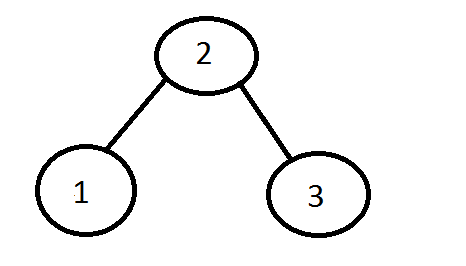
\includegraphics[width=1.5in, height=1.5in, scale=1, angle=0]{binary-tree.png} \end{center}
\end{enumerate}
\textsc{setlX} supports 3 main functions for terms.
\begin{enumerate}
\item \texttt{fct(t)} which returns the functor of a term $t$.
\item \texttt{args(t)} which returns the arguments of a term $t$.
\item \texttt{makeTerm(f,l)} which creates a term of functor $f$ and arguments $l$.
\end{enumerate}
So executing \texttt{fct(Node(3,Nil(),Nil()))} yields a result of \texttt{"Node"},\\
and executing \texttt{args(Node(3,Nil(),Nil()))} yields a result of \texttt{[3, Nil(), Nil()]},\\
and executing \texttt{makeTerm(\symbol{34}Node\symbol{34},[ makeTerm(\symbol{34}Nil\symbol{34},[]), makeTerm(\symbol{34}Nil\symbol{34},[]) ])} constructs the term \texttt{Node(3, Nil(), Nil())}.
\\
\\
Figure \ref{fig:binary-tree-no-matching.stlx} actually shows how terms can be used in \textsc{setlX} to implement binary trees.
\pagebreak
\begin{figure}[!ht]
\centering
\begin{Verbatim}[ frame         = lines, 
                  framesep      = 0.3cm, 
                  firstnumber   = 1,
                  labelposition = bottomline,
                  numbers       = left,
                  numbersep     = -0.2cm,
                  xleftmargin   = 0.8cm,
                  xrightmargin  = 0.8cm,
                ]
    insert := procedure(m, k1) {
        switch {
            case fct(m) == "Nil" : 
                 return Node(k1, Nil(), Nil());
            case fct(m) == "Node": 
                 [ k2, l, r ] := args(m);
                 if (k1 == k2) {
                     return Node(k1, l, r);
                 } else if (compare(k1, k2) < 0) { 
                     return Node(k2, insert(l, k1), r);
                 } else {
                     return Node(k2, l, insert(r, k1));
                 }
        }
    };
\end{Verbatim}
\vspace*{-0.3cm}
\caption{Inserting an element into a binary tree.}
\label{fig:binary-tree-no-matching.stlx}
\end{figure}

\subsection{Statements in \textsc{setlX}}











\end{document}